\section{Model Checking the CCUCprotocol}
This section will utilise UPPAAL to see what happens with the model when unreliability is introduced to the model.

The changes to the model are that whenever something is received, it will have a chance to miss the transmission, and therefore not fire the edge which receives the transmission.
This can be modelled in UPPAAL using the branch points as seen on \myref{fig:missTransmission}.

\begin{wrapfigure}{R}{0.3\textwidth}
\centering
  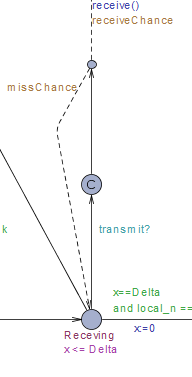
\includegraphics[width=0.3\textwidth]{Figures/Model/MissChance.png} 
\caption{Model in UPPAAL showing the split node after receiving, where there is a chance for the device to miss the transmission and go back to the same location.}
\label{fig:missTransmission}
\end{wrapfigure}

The chances \texttt{missChance} and \texttt{receiveChance} are simply created so the sum of them is 100 and this is shown in \myref{unreliability-UPPAAL}.

\begin{lstlisting}[style=UPPAAL, caption={Specifying the realiability of the transmissions, the current numbers result in a 2\% miss chance.}, label={unreliability-UPPAAL}]
//States how reliable the network is
const int receiveChance = 98;
const int missChance = 100 - receiveChance;
\end{lstlisting}

When the branch points are used everywhere a transmission could be received before, the devices will have a miss chance on every transmission received much like in the real world examples, as with the Arduinos and the RF modules used for this project.
To see the effect of these changes the query from earlier which tests if a network is succesfully created can be used, the query can be seen on \myref{query-SuccesfulCreate}.

\begin{lstlisting}[style=UPPAAL, caption={Query for UPPAAL which asks for the probability of all devices in a network being equal to the number of devices in the system, and that they all have the same \texttt{network\_id}}, label={query-SuccesfulCreate}]
Pr[<=300000] ( <>  forall(i: id_t) forall(j: id_t) (time >3000) 
	and  ((Device(i).local_n == N+1 
		and Device(i).local_network_id == Device(j).local_network_id)))
\end{lstlisting}

With a confidence of 99\% the probability range lies in the range [0.933723, 0.95372], which means that the somewhere in that range lies the probability of a succesful network being created.
This means that the impact of this reliability is actually quite large, and something should be done.
As stated earlier in \myref{??}\todo{KILDE TIL CCUC DESIGN}, one could make the devices transmit more than once in order to reduce the chance of a transmission being completely missed.
To make this further changes to the model is required.
Whenever a transmission is sent, it should be able to loop in the same location for the number of times it should transmit, before finishing its time-slot. 
This also means that the time-slots' length will have to be increased to make up for the increased transmission time.
One of these loops can be seen on \myref{LoopTransmitUPPAAL}.

\begin{wrapfigure}{R}{0.5\textwidth}
\centering
  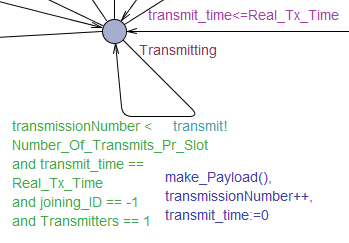
\includegraphics[width=0.5\textwidth]{Figures/Model/Transmit_Loop.png} 
\caption{Model in UPPAAL showing the loop, where it transmits for the amount of times specified minus one. The last transmission in a time-slot will occur when it finally leaves the location.}
\label{LoopTransmitUPPAAL}
\end{wrapfigure}

This also requires changes to the code in UPPAAL, which can be found in \myref{UPPAAL-CCUC-Code}, and also on the attached CD.
The complete model for the CCUC-protocol can also be found printed on a A3-paper in the back of the report.

The model has then been tested with the query seen in \myref{query-SuccesfulCreate}, with varying miss chance, and with varying number of transmissions in a time-slot.
This should show how the change of transmitting more than once would efffect the model.

The results of this test can be seen on \myref{CCUC-Graph-UPPAAL}.

\begin{figure}[ht]
  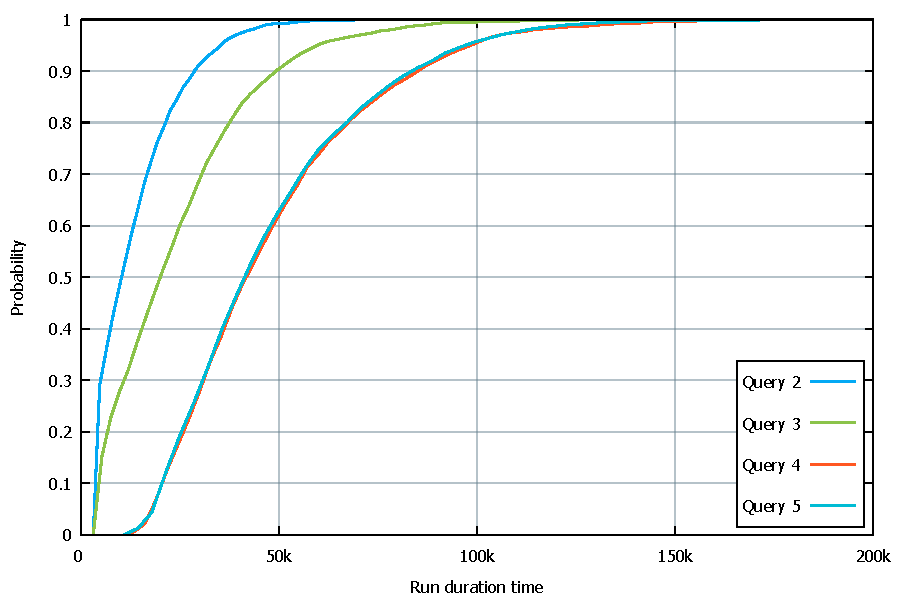
\includegraphics[width=1\textwidth]{Figures/Graphs/gnuplot/uppaal/graph.pdf} 
\caption{Block-diagram of the query that requires a succesful network creating, with varying miss chance, and varying number of transmissions.}
\label{CCUC-Graph-UPPAAL}
\end{figure}
\todo[inline]{Sass er i gang med at lave den rigtige figur... HUSK AT ÆNDRE DEN}

The results shows that transmitting more than once is actually a viable option as most times the network will actually be created succesfully and correct.
The problems with unreliability do however lie in the creation of the network, as the model in uppaal will work correctly in the main loop.
This was tested by instantiating a network of 4 devices which were when the system started all connected to the same network, and had been given different $k$ values. 
This means that a network is succesfully created.
A query was asked to this system, which can be seen on \myref{stable-network-query}.

\begin{lstlisting}[style=UPPAAL, caption={Query for UPPAAL asking if for all devices i and j, when they are in the location \texttt{User\_Code} will they have they then have the same value for \texttt{local\_i}.}, label={stable-network-query}]
Pr[<=300000] ( <> forall(i: id_t) forall(j: id_t)  (time >3000) 
	and ((Device(i).User_Code and Device(j).User_Code) 
		imply (Device(i).local_i == Device(j).local_i)))
\end{lstlisting}
The results of the query will be a probability in the range [0.980056, 1] with a confidence of 99\%, which means that the problem truly does lie in connecting to the network, with unreliable transmission.

